%!TEX root = ../template.tex
%%%%%%%%%%%%%%%%%%%%%%%%%%%%%%%%%%%%%%%%%%%%%%%%%%%%%%%%%%%%%%%%%%%%
%% chapter4.tex
%% NOVA thesis document file
%%
%% Chapter with lots of dummy text
%%%%%%%%%%%%%%%%%%%%%%%%%%%%%%%%%%%%%%%%%%%%%%%%%%%%%%%%%%%%%%%%%%%%
\chapter{Background}
\label{cha:background}
This thesis aims to improve the interface that allows users to build queries in a more efficient and effective way. Therefore, \gls{HCI} is a core subject of the work since such an interface can only be improved if its interaction and usability in the user perspective are studied.

Accordingly, this chapter will introduce key concepts of \gls{HCI}, as well as, a brief contextualization of the OutSystems Platform that is indispensable for the comprehension and progression of this study.

\section{Human-Computer Interaction}
\label{sec:human_computer_interaction}
Although computer systems have been designed by humans, these two parts of \gls{HCI} do not speak the same language. Nonetheless, these types of systems were created to support, in a transparent way, human tasks and requirements, forgiving careless mistakes \cite{humanComputerInteraction}. Thus, \gls{HCI} aims to study the relationship of users and computer systems, in the context of the users’ desired tasks, in order to “unfold and reveal challenges and insights, and to instrument appropriate solutions for alleviating the current obstacles to the access and use of advanced information technologies” \cite{userInterfacesForAll_newPerspectivesIntoHumanComputerInteraction}. 

%\textit{Dix et al.} \cite{humanComputerInteraction} reinforce this too, saying that “HCI involves the design, implementation and evaluation of interactive systems in the context of the user’s task and work”.

%\subsection{Interaction Models}
%\label{subsec:interaction_models}

%Therefore, interaction models have been proposed to represent the intention of a user to perform a certain task on a system. One of the most influential is Norman’s model, that characterize the interaction of a user with a system beyond execution-evaluation cycles. \cite{humanComputerInteraction} Thereby, the execution is a flow when the user interacts with the system, and the evaluation phase comprises the presentation and the interpretation of the system output. However, this model only represents the interaction from the users’ point of view. Thereupon, Abowd and Beale \cite{userSystemsAndInterfaces_aUnifyingFrameworkForInteraction} proposed an extension of this model where it is possible to view how the system communicates through the interface.

%In this approach, represented in Figure \ref{fig:abowdAndBealeModel}, after the user has defined his goal and respective tasks to achieve it, he transmits his intention (articulation) through input language, and after this, that information is translated to system language (performance), ending the execution phase. Secondly, the result of the action executed by the system is presented (presentation) and the user observes it (observation), ending the evaluation phase.

%\begin{figure}[htbp]
%	\centering
%	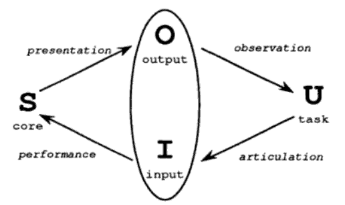
\includegraphics[height=1.75in]{abowdAndBealeModel}
%	\caption{Interaction Model proposed by Abowd and Beale \cite{userInterfacesForAll_newPerspectivesIntoHumanComputerInteraction} (Based on Norman’s Model)}
%	\label{fig:abowdAndBealeModel}
%\end{figure}

%These models are useful to understand two concepts that cannot be forgotten when a system is being designed, since these are two effects that designers want to reduce as much as possible, in order to optimize the effectiveness of the human-computer dialogue. Following, these concepts will be described respecting \textit{Dix et al.} \cite{humanComputerInteraction} definition:

%\begin{itemize}
%    \item \textbf{Gulf of execution}: “Difference between the user’s formulation of the actions to reach the goal and the actions allowed by the system. If the actions allowed by the system correspond to those intended by the user, the interaction will be effective.”
%    \item \textbf{Gulfs of evaluation}: “Distance between the physical representation of the system state and the expectation of the user. If the user can readily evaluate the presentation in terms of his goal, the gulf of evaluation is small.”
%\end{itemize}

\subsection{Main Concepts}
\label{subsec:main_concepts}
The \textbf{Usability} of a system is one of the most important concepts in \gls{HCI}, that can not be forgotten on the design process, since its attributes must be taken into account performing also a guidance function through all this process. This concept was standardized in ISO-9241 \cite{iso9241-11_2018} as “extent to which a system, product or service can be used by specified users to achieve specified goals with effectiveness, efficiency and satisfaction in a specified context of use”.

However, usability is not a single-dimensional property, being always associated with its attributes, that characterize the user accessibility when is using the system into five different points, such as referred by Nielsen \cite{usabilityEngineering}:

\begin{itemize}
	\item \textbf{Learnability}: How easy is the learning process until a novice user (who has not used the system before) achieves a high-level of proficiency using the system \cite{measuringLearnabilityInHumanComputerInteraction}. %The learnability is higher as the learning process is faster, and the user has to spend less effort to reach his goal. Also, it depends on the tutorials and training provided to users. A system that requires less training has higher learnability than a system that requires more training. The time that a novice user requires to perform some specific tasks can be used to measure learnability. Learnability can be improved using tips while a novice user explores the system doing his first tasks.
	\item \textbf{Efficiency}: Refers to the productivity level of a user who has already learnt how to use the system. %Efficiency can be measured analysing the time that expert users spent to do specific tasks on the system. This attribute can be improved, for example, adding shortcuts to accelerate the interaction process.
	\item \textbf{Memorability}: Defines how easy is for a user, that was using a system before but did not use it for a time period, to do his desired tasks on the system. %So it’s related to how many times the user has not used the system and the time that the user needs to remember how the system works. Therefore, if a system has good memorability the user does not need much time to remember it, even if it has stopped using it for a long period of time. Memorability can be measured, for example, analysing the interaction process of a user who has been away from the system, while he uses the system again. The use of visual components and metaphors with real-life objects helps, sometimes, the users in this process.
	\item \textbf{Errors}: A system not only must have a low error-rate but if an error occurs, the user should be able to recover from that. %Since there are multiple types of errors with different severity levels, catastrophic errors should not occur. This attribute can be measured by the evaluation of the error-rate, taking into account the severity levels of the errors. Furthermore, if a system has errors, that can be reverted and does not have a negative impact on the final result, cannot be forgotten that these errors also harm the efficiency of the system.
	\item \textbf{Satisfaction}: The most subjective attribute of the usability that is related to the overall satisfaction of the user when uses the system. %It could be measured by asking the users about the experience while they are using the system, always searching for subjective answers.
\end{itemize}

Nonetheless, as mentioned by Nielsen \cite{usabilityEngineering}: \textbf{“it is not always possible to achieve optimal scores for all usability attributes simultaneously”}. Thus, when a system is designed it is necessary to prioritize what are the most important attributes for the users and the domain where the system will be used and applied. These trade-offs are one of the most challenging tasks of the design processes because it depends on user expectations and their backgrounds, as well as, the problem domain and what are the main focus of the system use. Accordingly, it is fundamental that the design process can focus on target users of the systems. Therefore, the main concepts, processes, and techniques for a design process centered on the users will be described.

%\begin{center}
%	\textbf{“it is not always possible to achieve optimal scores for all usability %attributes simultaneously”}.
%\end{center} 





\subsection{User-centered Design}
\label{subsec:user_centered_design}
Before user-centered design principles and methodologies were adopted, the Waterfall model was commonly adopted as a software development process. This model comprises five sequential phases, from the requirements specification phase to the operation and maintenance phase, and has a good quality control since documentation and planning are a major concern of this methodology \cite{aComparisonBetweenThreeSDLCModelsWatterfallSpiralIncrementalIterative}. However, the stages of this model are not overlapping stages, so other development methodologies and philosophies arose to mitigate this problem and include the user on the design process, due to their impact on the usability of the system.

Consequently, it was necessary a new model that has the users included in the development process to verify, along with the development, if the approaches adopted are positive and what is the users' acceptability. Nielsen \cite{iterativeUserInterfaceDesign} reinforces this saying that “user interfaces should be designed iteratively in almost all cases because it is virtually impossible to design a user interface that has no usability problems from the start. Even the best usability experts cannot design perfect user interfaces in a single attempt, so a usability engineering lifecycle should be built around the concept of iteration”.

The Spiral model of iterative design arose as an iteration through design, implementation and evaluation phases where the cost and accuracy increase on each iteration. The first iterations should use low-cost resources, like paper prototypes, and when the results are positive the accuracy should be incremented, changing to high-fidelity prototypes, such as computer prototypes \cite{interactionDesign_beyondHumanComputerInteraction}. %An overview of this model is represented in  Figure \ref{fig:spiralModel}.

%begin{figure}[htbp]
%	\centering
%	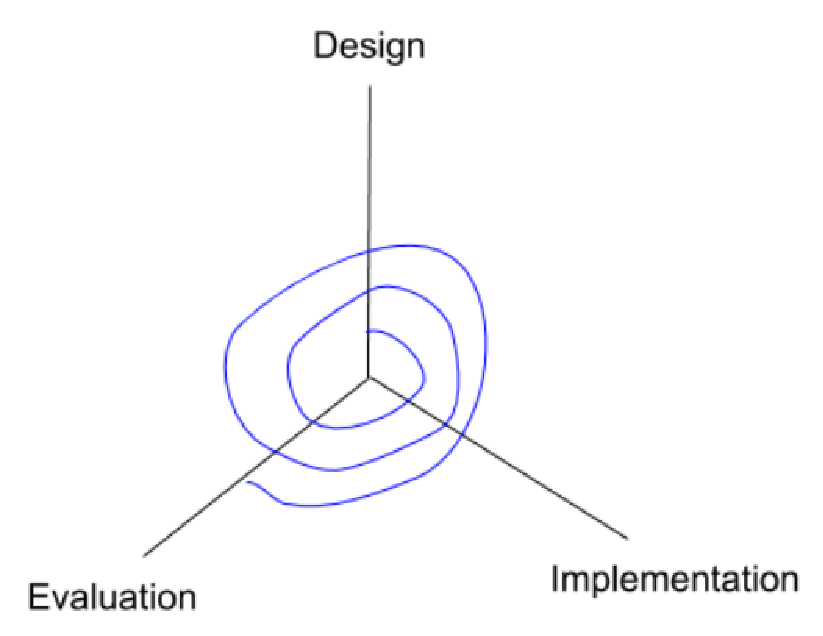
\includegraphics[height=1.75in]{spiralModel}
%	\caption{Sprial model of Iterative Design (adapted: \cite{interactionDesign_beyondHumanComputerInteraction})}
%	\label{fig:spiralModel}
%\end{figure}

\subsubsection{User and Task Analysis}
\label{subsubsec:user_and_task_analysis}
Regarding the concept of usability presented above and the importance of the users on the design process, it is important to define the users and their desired tasks of the system in order to find the best solution as possible to the usability attributes trade-offs. Just a good description of the users and the tasks of the system leads the designers to the best choice of what are the usability attributes most important for the system.

Accordingly, it is important to make a \textbf{User Analysis} to understand all users’ characteristics that could have an impact on the acceptability of the system. The expected result of this analysis should be a set of structured information that characterize the users of the system in terms of technological expertise, knowledge of the business domain, application experience, educational background, gender, and age, as other aspects that might be useful to comprehend, depending on the system’s users and domain \cite{userAnalysisInHCI_theHistoricalLessonFromIndividualDifferencesResearch}. The more traditional process to gather this information is through questionnaires or interviews, but that can also be obtained by conducting market analyses or observational studies \cite{usabilityEngineering}.

Furthermore, it is essential to enumerate and analyze the tasks the users should perform using the system. The \textbf{Task Analysis} process aims to aggregate information about the tasks that should be performed on the system, starting from the system's overall goals and break down these to obtain individual tasks \cite{usabilityEngineering}. Moreover, the goal of this analysing process is to obtain more structured information about: how the tasks are performed using the existing systems, what are the pre-conditions and the requirements of each task, why the users need to perform this tasks, and others that might be useful to characterize the tasks of the system. 

The techniques used, to extract information to this analysis, aims at figuring out how the tasks should be done instead of how they would perform them. The idea is to resort to examples, as well as possible, in order to understand what type of strategies are used, what type of exceptions from their normal workflow is occurring, and other aspects that can be observed where the communication with users is on a concrete level \cite{usabilityEngineering}. In addition, Nielsen \cite{usabilityEngineering} points out that  “The users' model of the task should also be identified, since it can be used as a source for metaphors for the user interface”, which reinforces that these dialogues with users to obtain analysis content, can be useful also to find relevant solutions to latter design process phases.

Therefore, the outcome of this analysis should contain a list of the entire tasks that users what to perform in the system, the information that is required to complete them, the steps and the dependencies between tasks, all the outputs that must be generated, and how is the communication process between the users associated with the system’s tasks \cite{usabilityEngineering}.


\subsubsection{Sketching and Prototyping}
\label{subsubsec:sketching_and_prototyping}
After the user and task analysis process, designers must start sketching and prototyping ideas and approaches, in order to think about how can they solve the problems. Nevertheless, this phase of the design process should start with sketching techniques, as these are not only a good and inexpensive starting point to communicate ideas, but also help to develop structure and enrich the reasoning, leading to the perception of other details as well as of other approaches to solving the related problems.

While sketching techniques are more plentiful, and have a low detail level, being mainly based on suggesting and exploring, rather than retrieving results, the prototyping phases, have more refinement approaches and are used to test the design choices made.

However, prototypes may have different thoroughness degrees, presenting different advantages and disadvantages. Thus, it is important to start the prototyping process with low fidelity prototypes, as paper prototypes, since the objective of these is to evaluate the conceptual model (if the users understand the system), the functionalities presented, the navigation, the screen components distribution, and the terminology used. After the evaluation of these prototypes presents good results, high fidelity prototypes should be used, like computer prototypes. There are a set of available tools to assist in the building process of these prototypes, such as Balsamiq \cite{balsamiq} and Mockingbird \cite{mockingbird}. These different prototype types can detect different issues when tested with users, so it is very important to test prototypes with different granularity levels.

Furthermore, there is another relevant aspect of the prototype designing, that is the scope definition of the prototype. It is important to define what features the prototype undertakes and what is the inherent detail level. Nielsen \cite{usabilityEngineering} describes this as two dimensions of prototyping: horizontal prototyping and vertical prototyping. %, as demonstrated in Figure \ref{fig:prototypeDimensions}. 
A vertical prototype is characterized as a prototype to test a restricted part of the system but with real users and circumstances. A horizontal prototype is presented as suitable for test the entire system but in a less realistic approach.

%\begin{figure}[htbp]
	%\centering
	%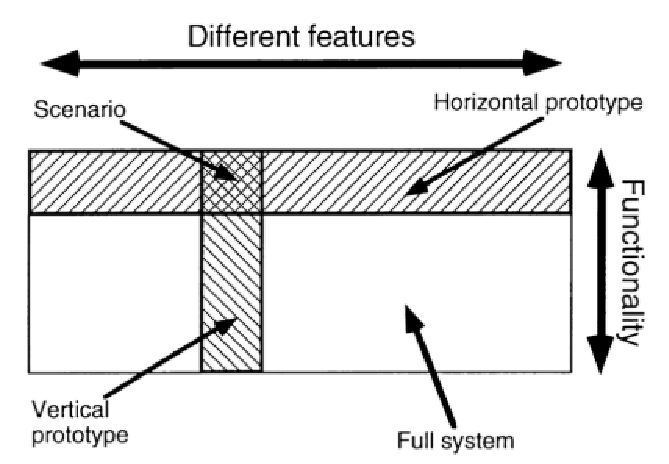
\includegraphics[height=2.5in]{prototypeDimensions}
	%\caption{The two dimensions of prototyping: Horizontal prototyping keeps the features but eliminates depth of functionality, and vertical prototyping gives full functionality for a few features (extracted from \cite{usabilityEngineering})}
	%\label{fig:prototypeDimensions}
%\end{figure}

Finally, regarding the methodology about how to use the prototypes built, Dix et al. \cite{humanComputerInteraction} refer that are three main approaches:

\begin{itemize}
	\item \textbf{Throw-away}: After the prototype is built and tested, it is used on the final system development, but after that, the prototype is discarded and the rest of the design process continues without relying on the prototype previously built;
	\item \textbf{Incremental}: First, the system is separated into different parts, and each part is built, one at a time. So the prototypes are developed separately, regarding its correspondent part, and finally are combined to build the final system;
	\item \textbf{Evolutionary}: Contrary to the throw-away approach, the prototypes developed are used as the basis for the next iteration of the design.
\end{itemize}





\subsubsection{Evaluation Techniques}
\label{subsubsec:user_and_task_analysis}
The evaluation phases are crucial in the design process, since they allow designers to understand the systems' specific problems and the impact of the interfaces on users. So, the expected outcome of these processes is a list of usability issues ordered by priority level, referring to what usability principles and guidelines are not being accomplished and what solutions can be applied to solve the problem \cite{usabilityEngineering}.  

However, there are different approaches to evaluate interfaces. First, one important topic that distinguishes two types of techniques is who performs the evaluation. There are techniques where only the designers and specialists are involved in the process and are another type of evaluation where users participate in \cite{humanComputerInteraction}. Thus, there are two types of evaluation: evaluation through expert analysis and evaluation through user participation.

\bigskip

\textbf{Evaluation through expert analysis}

In this type of evaluation, designers, or other specialists, evaluate the system, supporting their analysis on cognitive principles, to preview usability problems likely to occur. Moreover, this evaluation not only is cheaper because it does not involve users, as it also can be applied to any phase of the design process, from the design specification to the high fidelity prototypes \cite{humanComputerInteraction}.

Regarding the approach presented above, these two methods are one of the most used:

\begin{itemize}
	\item \textbf{Heuristic Evaluation} \cite{heuristicEvaluationOfUserInterfaces}: The system is thoroughly analyzed in order to find problems that do not follow importantly and recognized usability heuristics. After a problem has been detected, it should be reported, not only with a description of the problem but also the indication of the heuristics that have not been accomplished, the severity level of the problem and possible solutions to solve it \cite{usabilityEngineering}.
	\item \textbf{Cognitive Walkthrough} \cite{cognitiveWalkthroughs}: This method uses a sequence of actions as the principal resource to guide the evaluation process. For each action, the evaluator tries to understand if all steps are clear and visible, as well as, if the system gives clear feedback, confirming if the action has been completed. Usually, the main focus of this method is to analyze the learnability of the system. Mainly, to understand if the system provides a good learning mechanism through exploration, rather than using manuals, training or other types of \textit{a priori} learning processes \cite{humanComputerInteraction}.
\end{itemize}

A study made by Desurvire \textit{et al.} \cite{WhatIsGainedAndLostWhenUsingMethodsOtherThanEmpiricalTesting} concluded that Heuristic Evaluation made by specialists is better to predict some problems before the user testing process than Cognitive Walkthrough. The reason pointed out for this result is that heuristic evaluation can often help to remind the designers of problems since this method analyses more dimensions of the system than Cognitive Walkthrough.

\bigskip

\textbf{Evaluation through user participation}

Although there exist methods that do not need the users to evaluate the system usability, it is difficult to predict all the behaviors of the users when they interact with a system. Therefore, there are multiple methods to make usability tests with people that are the system's target. Some methods of user testing which can be resourceful on the context of this work, are the following, respecting the terminology used by Dix \textit{et al.} \cite{humanComputerInteraction}:

\begin{itemize}
	\item \textbf{Observational Methods}: the main principle of these methods is observing users using the system to conclude important usability information about it. %Usually, it is requested to the user to ‘thinks aloud’ since it might be possible to obtain more insights that can be useful, not only to understand why the user might have made an error, but also it can be a good strategy to find starting points for other possible solutions. Moreover, although usually, these tests have a set of predetermined tasks, since it is easier to find the user reaction to the system part the need to be tested, also can be executed tests only by evaluating the normal tasks of the users on their work;
	\item \textbf{Experimental Methods}: starting from a properly defined test hypothesis, it is selected a set of users to perform an experimental test to verify if the test hypothesis proves to be true or not. %Thus, it is necessary to define previously all the experimental environment, which includes: the test hypothesis that wants to be verified, the users that will perform the test,  and the independent and dependent variables. The dependent variables are the ones that express the result of the test in  function of the independent variables, such as the task execution time or the number of the errors that occurred. The independent variables are chosen by the test designer to produce different conditions for comparison. Examples of independent variables can be the size of an interface component or the use of an interaction technique. This method is very useful to verify through a test hypothesis which of the possible solutions presented (independent variables) have a better performance for the intended application context;
	\item \textbf{Query Methods}: these methods focus on what the users think about the system, collecting information from interviews or questionnaires to analyze their opinion. %One advantage of this method is that it might reveal issues not observed previously complained before, but contrary a lot of cases are not tested, since in the interaction field, many times, the user only finds a problem when it occurs for the first time. So it is not possible to extract concrete information from users that never have passed for this situation.
\end{itemize}

%\bigskip

%Finally, independently of the evaluation process adopted (through expert analysis or user participation), severity ratings should be attributed to the problems identified in order to define the main priorities and understand which might have a larger impact on the system acceptability. However, although these levels should be attributed by specialists, if they use not only cognitive principles, but also use the results observed from the user testing phase to sustain the classification of the problems detected, the result can be more accurate. 

%Besides, the Figure \ref{fig:severityLevels}, extracted from \cite{usabilityEngineering}, displays two influential factors that should be taken into account to attribute a severity level to a problem: how many users are experiencing this problem and what is the impact level on the user.

%\begin{figure}[htbp]
%	\centering
%	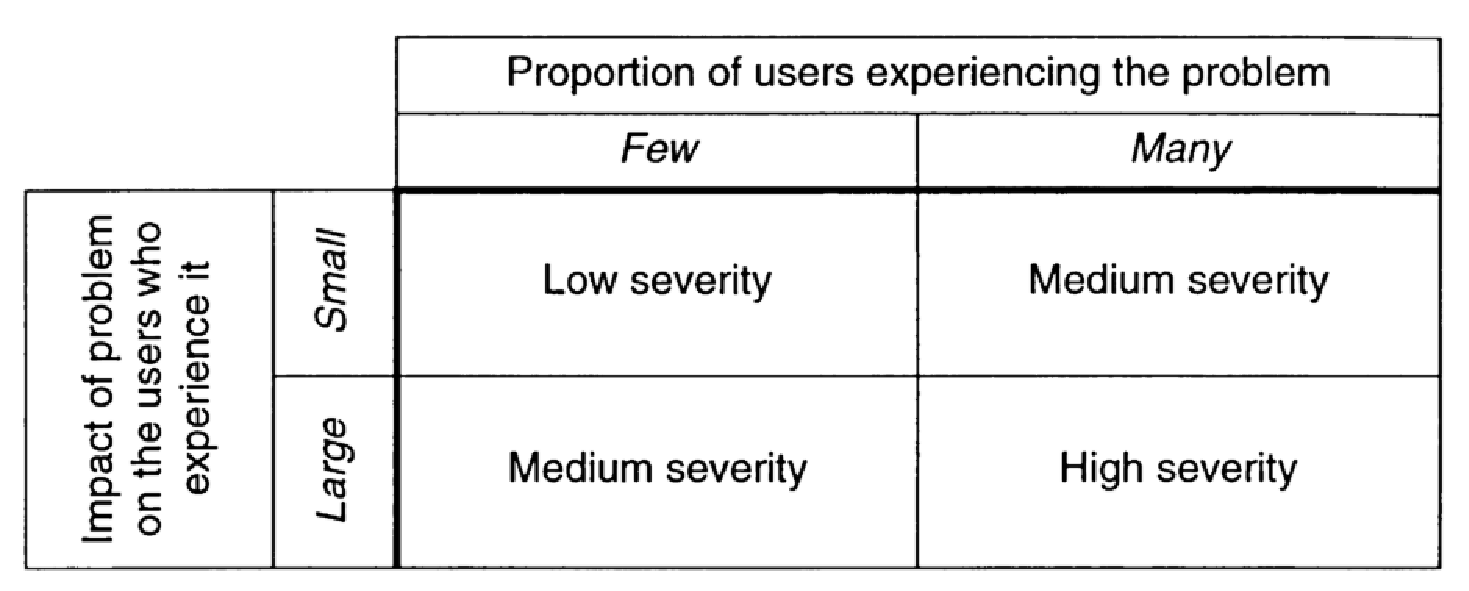
\includegraphics[height=2in]{severityLevels}
%	\caption{Severity Levels of the Problems based on their impact on the users (extracted from \cite{usabilityEngineering})}
%	\label{fig:severityLevels}
%\end{figure}

%\subsubsection{Errors Classification}
%\label{subsubsec:errors_classification}
%The errors that occurred when a user interacts with a system are excellent indicators to designers because the understanding of the reason that led to error situations is a good strategy to classify them. Therefore, errors can be classified as slips and mistakes, as will be presented below according to Dix \textit{et al.} \cite{humanComputerInteraction}:

%\begin{itemize}
%	\item \textbf{Slips}: in these types of errors, the user knows how to do the intended task on the system, however, he presses a wrong button or closes one window accidentally. So, he understands the action, but a misaction does not allow that he reaches his goal;
%	\item \textbf{Mistakes}: these errors occur when the user does not understand the system, formulating a wrong goal. An example of a mistake is when the user does not understand the action associated with an icon, performing a not intended action.
%\end{itemize}

%Therefore, the strategy to mitigate the problems associated with these two types of errors could be different, as mentioned by Dix \textit{et. al.} \cite{humanComputerInteraction}: “Slips may be corrected by, for instance, better screen design, perhaps putting more space between buttons. However, mistakes need users to have a better understanding of the systems, so it will require far more radical redesign or improved training, perhaps a totally different metaphor for use.”


\section{OutSystems Background}
\label{sec:outsystems_background}

The OutSystems Platform has the mission of simplifying and accelerating the development and management of digital enterprise solutions, no matter the dimension and domain of the applications. It covers the entire development lifecycle which aims to promote rapid development and integration, to facilitate and speed up the deployment stages, to keep track of the status and health of the applications produced, and to expedite the management of daily operations and configurations on the final products \cite{eg_developingWithOutsystems}.

\subsection{Visual Development Environment}
\label{subsec:visual_development_environment}

Service Studio is the low-code development environment of the platform, which allows the developers to create complete applications using visual elements to perform drag and drop actions. Figure \ref{fig:ss_workspace} presents an overview of the \gls{IDE}, which highlights the different areas of the workspace.

\begin{figure}[tb]
	\centering
	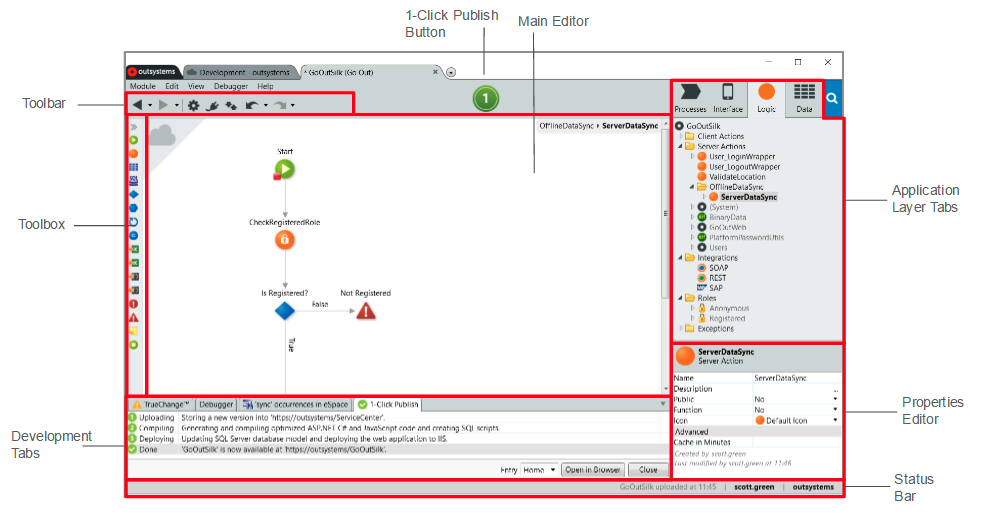
\includegraphics[height=3.1in]{ss_workspace}
	\caption{Main areas of Service Studio (source: OutSystems\cite{serviceStudioOverview})}
	\label{fig:ss_workspace}
\end{figure}

Using the widgets and icons provided in the toolbox, the main area is dedicated to designing the applications’ interface and logic. So, in the main area, there are visual elements, which can be set using the properties editor, placed on the bottom right corner of the screen. 

Also, it includes other sections whose main purpose is not the product development, but are related to key actions of the software development process. Therefore, on the window’s top, there is a toolbar which has shortcuts to some of the most common operations, and a green circle button, denominated "1-Click Publish button", to start the automated deployment process provided. Besides, the bottom of the window is dedicated not only to the presentation of messages, errors, and warnings but also to debugging the application.

Since the development environment can be used to develop a complete full-stack application, the elements, which can be manipulated in the Service Studio, can be related to different parts of the application. The Application Layer Tabs, which contain a tree view of its elements, are the following:

In the \textbf{Processes} tab is possible to create and manage business processes of the systems through a flow that can be composed by human or automatic activities, time waits, conditional decisions and indications to execute processes. In addition, this section can be used to configure the timers of the application. Then, it is possible to indicate when a timer should start, what is it period and what action should be performed when it is triggered.

The \textbf{Interface} tab can be used to manage the components related to the visual interface of the final application. It is possible to observe all applications’ screens, as well as, the variables and the actions related to each one. Moreover, flows between the various screens can be also defined. If one screen or action is selected, it will be possible to add new visual components to the interface or assign new elements to the action flow in order to define all the client-side logic of the screen.

The \textbf{Logic} tab is where the core logic of the application could be defined. It includes not only the server actions of the application but also the exceptions specification, the existing user’s roles and also the integration with external services. Although there is a data section on the application layer tabs, which will be described below, the actions which require data querying are managed in this section.

In the \textbf{Data} section is covered the database modelling, making possible the creation of diagrams to represent the schema of the database. Moreover, in the tree view of this tab is allowed to establish new entities and static entities in order to define the data model of the application.

%\begin{itemize}
%	\item \textbf{Processes}: in this section, it is possible to create and manage business processes of the systems through a flow that can be composed by human or automatic activities, time waits, conditional decisions and indications to execute processes. In addition, this section can be used to configure the timers of the application. Then, it is possible to indicate when a timer should start, what is it period and what action should be performed when it is triggered;
%	\item \textbf{Interface}: the purpose of this section is the management of the components related to the visual interface of the final application. It is possible to observe all applications’ screens, as well as, the variables and the actions related to each one. Moreover, flows between the various screens can be also defined. If one screen or action is selected, it will be possible to add new visual components to the interface or assign new elements to the action flow in order to define all the client-side logic of the screen;
%	\item \textbf{Logic}: the area where the core logic of the application could be defined. It includes not only the server actions of the application but also the exceptions specification, the existing user’s roles and also the integration with external services. Although there is a data section on the application layer tabs, which will be described below, the actions which require data querying are managed in this section.
%	\item \textbf{Data}: the database modelling aspects are covered in this section, making possible the creation of diagrams to represent the schema of the database. Moreover, in the tree view of this tab is allowed to establish new entities and static entities in order to define the data model of the application.
%\end{itemize}

\subsection{Visual Data Querying}
\label{subsec:visual_data_querying}

The main topic of this work is the improvement of the visual data querying process on the low-code development of applications, using OutSystems. Consequently, the headway of visual querying components of the platform is an essential factor to properly understand the entire project. Regarding the last version of the OutSystems platform, the actual visual data querying tool, which is the starting point of this study, will be described.

\subsubsection{Previous Work}
\label{subsubsec:previous_work}

Since 2002, which is the release date of the first OutSystems low-code development environment, the Hub Edition 1.0, allows two manners to create database queries \cite{whatsNotNewInOutsystems}:

\begin{itemize}
	\item \textbf{Simple Queries}: visual query builder that allows the creation of some less complex queries, interacting with a graphical user interface;
	\item \textbf{Advanced Queries}: feature to specify queries textually, using a language based on \gls{SQL}, but includes some extra syntax to reference variables used of the application development;
\end{itemize}

Then, since the first versions of the \gls{IDE}, it is provided two ways to build queries. The first uses the visual language, which does not need so many learning requirements but also diminishes the necessity to remember the entities' name or the language syntax. The second provided relies on \gls{SQL}, which is the standardized textual query language, known for the developers' majority.

The first simple queries versions have accelerated the query building process finding automatically the relationships between the entities chosen. The main idea is that the developer only needs to select the entities intended and the respective join conditions would appear automatically in the query view interface. After this, it will be possible to change the join type, as well as, to add, edit and remove filtering or sorting conditions. Figure \ref{fig:ss_simpleQuerieOuterJoinHub2} presents a simple query example in Hub Edition 2.0 (2003) when the developer was changing the join type to an Outer Join.

\begin{figure}[tb]
	\centering
	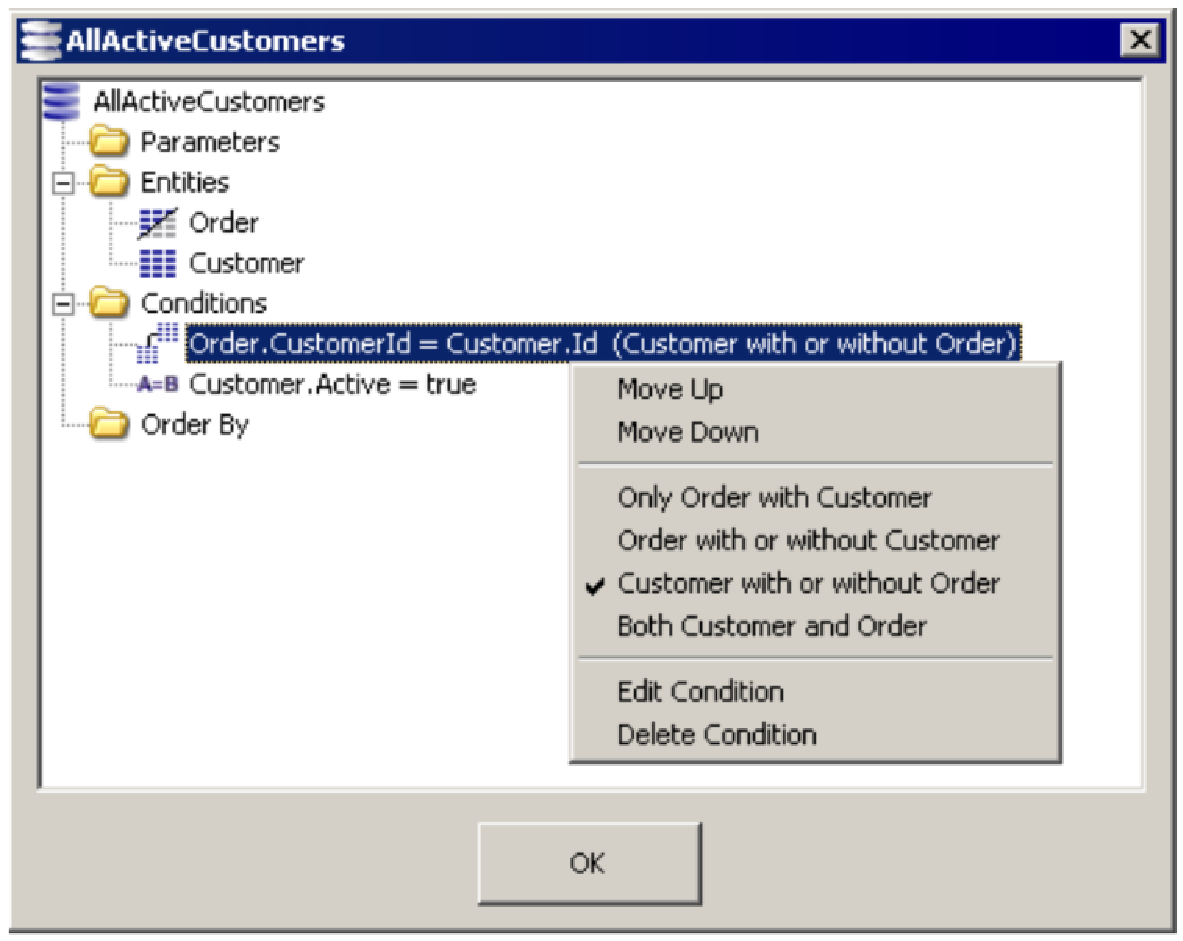
\includegraphics[height=2.6in]{simpleQuerieOuterJoinHub}
	\caption{Simple Query example in Hub Edition 2.0 (source: OutSystems \cite{whatsNewHub2})}
	\label{fig:ss_simpleQuerieOuterJoinHub2}
\end{figure}

This visual querying approach continued in the next versions, adding some minor improvements, such as the support to structures in order to store temporary information without changing the entity definition \cite{whatsNewHub22}, and the inclusion of a properties pane to view and change the properties of all query elements in a single window \cite{agilePlatform5}.

However, at the launch of the OutSystems Platform 9 (2013), an entirely new way to manipulate data and express database queries has been released. These new components of the system, called \textbf{Aggregates}, have replaced Simple Queries, promoting a new interaction strategy to query databases, where the main focus is the data, instead of query design. Also, new features have been introduced to improve the expressiveness of the \gls{VQL}, namely grouping functions and the ability to add calculated columns easier.


\subsubsection{Current Progress}
\label{subsubsec:current_progress}

Since the implementation of Aggregates, the query process without textual languages is more visual and more focused on the query outcome. Aggregates can be used to query data from the server or mobile local storage, and can be created in the following ways: ff someone is designing the user interface and wants to present some data gathered from the database (server or local storage), he can right-click on the screen where data will be displayed and select “Fetch Data from Database”; when an action flow is designed, there is an Aggregate icon in the toolbox that can be dragged and dropped to the main area;

%\begin{itemize}
%	\item If someone is designing the user interface and wants to present some data gathered from the database (server or local storage), he can right-click on the screen where data will be displayed and select “Fetch Data from Database”;
%	\item When an action flow is designed, there is an Aggregate icon in the toolbox that can be dragged and dropped to the main area;
%\end{itemize}

When the Aggregate is created, the first step is the data source selection in order to specify what entities should be included in the query. Then, the developer should click in the main area and choose the entities he wants or drag and drop the entities to add them to the query. When an entity is added, all its attributes are automatically included in Aggregate. Since an Aggregate can include one or more entities, added on the beginning or later, if it has more than one, it will be analysed to verify if there are relationships between them. Unless there is a relationship that links them, the Aggregate will request the condition to join them. Otherwise, the entities will be included automatically using an inner join.

%\begin{figure}[htbp]
	%\centering
	%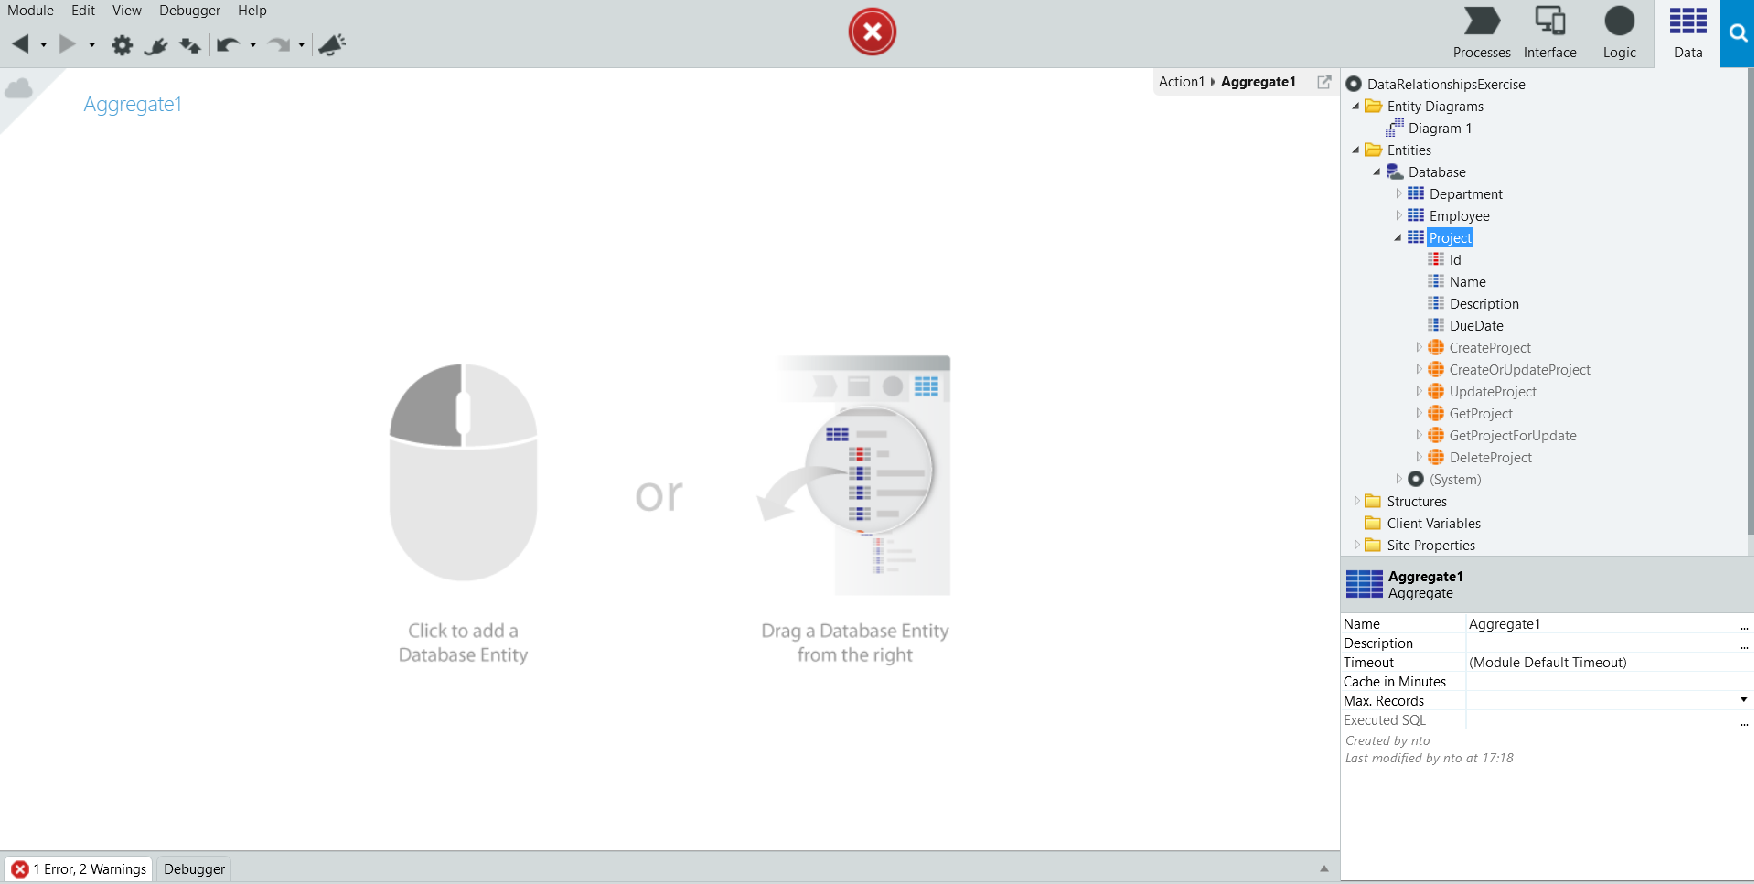
\includegraphics[height=2.8in]{aggregateCreated}
	%\caption{Aggregate Initial View}
	%\label{fig:aggregate_created}
%\end{figure}

Hereupon, the Aggregate has already been created and its data source specified, so the visual querying process can be started, in a progressive way, seeing at the same time the query output. Figure \ref{fig:aggregate_created} demonstrates an Aggregate on the referred state, to be possible to understand the structure of the interface.

\begin{figure}[tb]
	\centering
	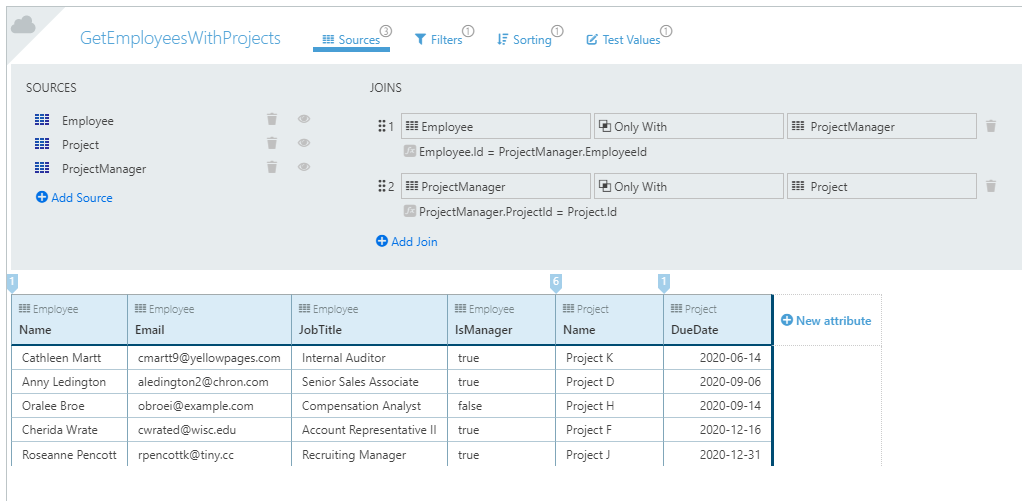
\includegraphics[height=2.7in]{aggregateExampleSource2}
	\caption{Aggregate Example}
	\label{fig:aggregate_created}
\end{figure}

First, this component of the OutSystems Platform presents two main capabilities, represented visually in two distinct areas: the query design area, and the viewer of the query result. The former, located at the top of the window, is composed of a set of four tabs, where each selection action changes the grey area to the respective form-based interface. The latter is a table-based interface, which is similar to spreadsheets applications, such as Microsoft Excel \cite{microsoftExcel} of Google Sheets \cite{googleSheets} and its principal aim is to provide a direct and visual approach to show the query output.

Focusing on the query design area, the sources tab, illustrated in Figure \ref{fig:aggregates_source_tab}, can be used to add, change or remove the entities of the quey, defining also, the join types between them. There are three join types available: "only with", "with or without", and "with". The respective joins in \gls{SQL} are: "inner join", "left join", and "full outer join". Additionally, each one appears with a visual representation similar to Venn Diagrams \cite{venn1880diagrams} to be easier to identify which data is selected on each join type. Moreover, it is possible to edit the join condition textually, using the platform expression editor.

\begin{figure}[tb]
	\centering
	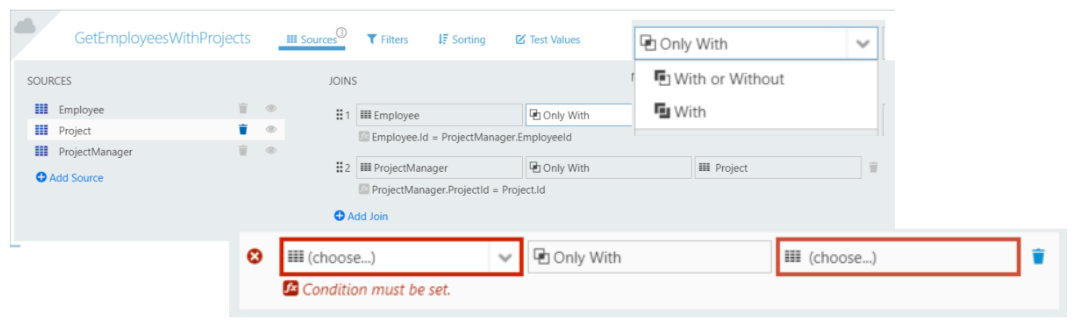
\includegraphics[height=1.7in]{aggregatesSourceTab}
	\caption{Aggregate - Defining Sources}
	\label{fig:aggregates_source_tab}
\end{figure}

The filtering tab can be used to apply filters in the query likewise the WHERE statements in \gls{SQL}. These filters can be defined through boolean conditions inserted in the expression editor. The conditions are specified textually with the assistance of some auto-completes and shortcuts available in a tree view. 

The sort conditions can be added in the sorting tab choosing the "add sort" or the "add dynamic sort" options available. The difference between them is that dynamic sort relies on a variable of the system, contrary to the other that depends only on an entity attribute. To add a sort, the user has to select what entity wants to sort and specify what are the sort criteria, for example, ascending or descending. Moreover, more than one sort can be inserted and they can be ordered to establish the priorities between them.

Finally, the last tab has a different behavior when compared with the rest of the options available in this interface area. The main goal of this feature is the testing of query output when concrete values are assigned to the variables referred to in the query. Thus, it does not contribute to the query design in the same way as the other tabs, presenting only a test purpose in the context of the query result visualization.

Figure \ref{fig:aggregates_filter_sort_test} presents a usage example of the last functionalities mentioned, to create a query to filter and sort dates, regarding the value of a variable.

\begin{figure}[tb]
	\centering
	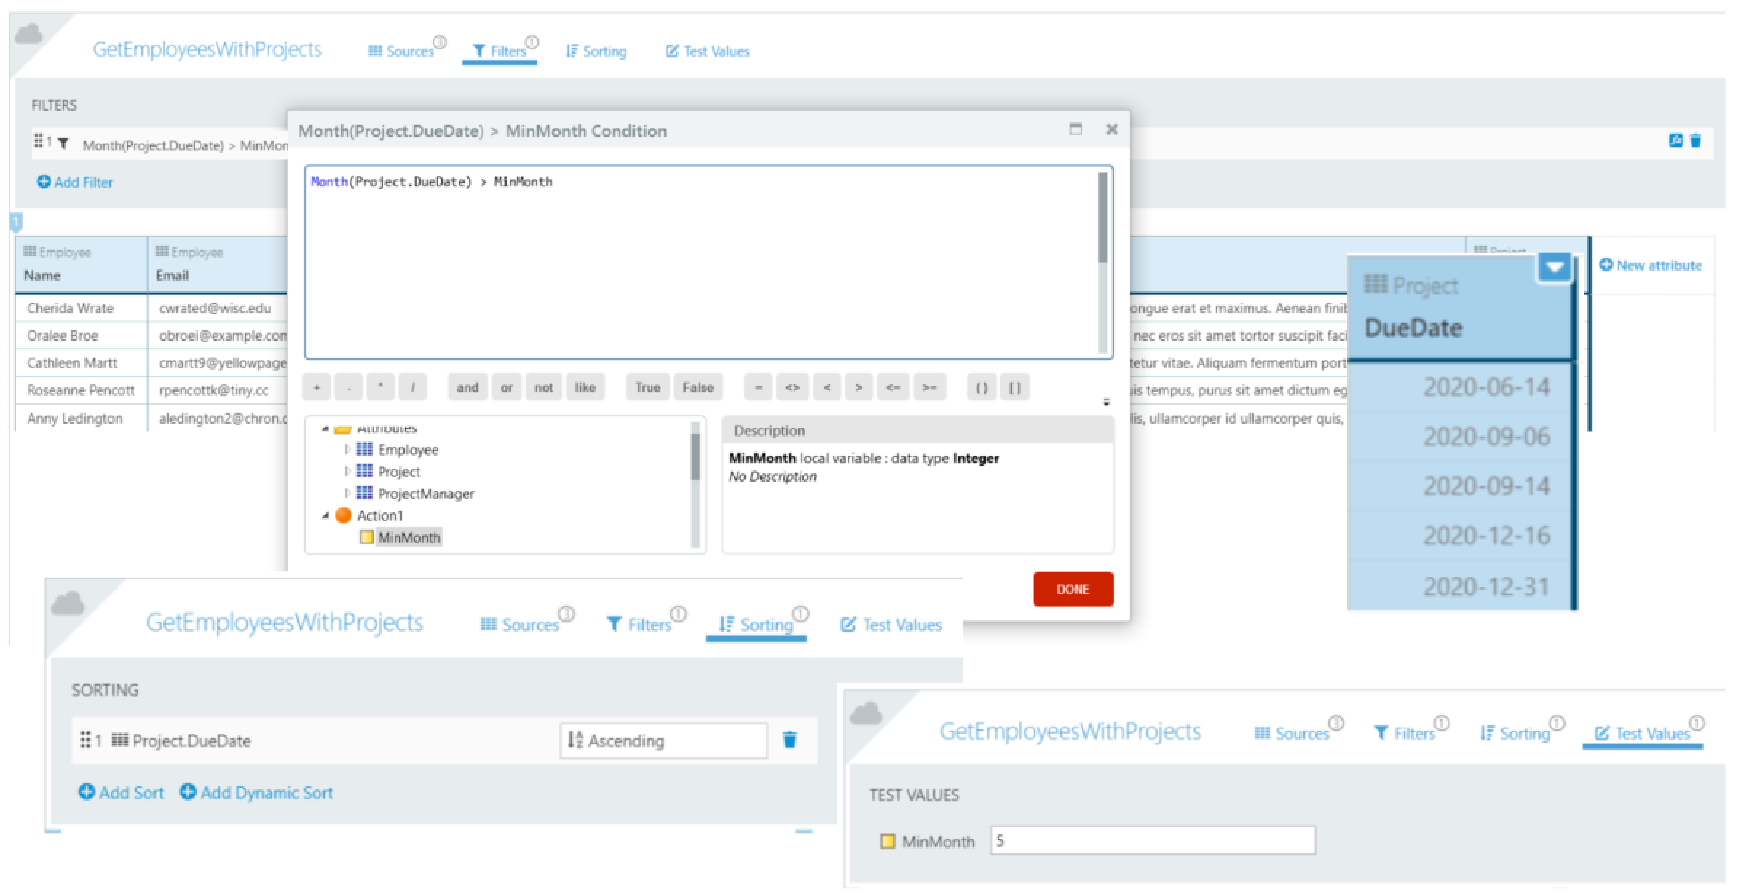
\includegraphics[height=2.8in]{aggregateFilterSortTest}
	\caption{Aggregates - Filtering, Sorting and Test Values in an example of querying DueDates after a month indicated in a variable}
	\label{fig:aggregates_filter_sort_test}
\end{figure}

On the other side, the area dedicated to viewing the query output provides also some functionalities to design the query while the user is interacting and exploring the query result. Therefore, as represented by an example in Figure \ref{fig:table_right_click_example}, the user can change the query when he performs a right-click on a column or when clicks on the new attribute. The only options in the list presented that does not change the query are the hide options since they just change the result in the presentation layer. So, if the user hides a set of columns, he will not see them in the result table, however, the query did not change. Besides, the user can add other attributes based on the existing ones, so Figure \ref{fig:calculated_attribute_example} shows an example of this functionality.

\begin{figure}[tb]
	\centering
	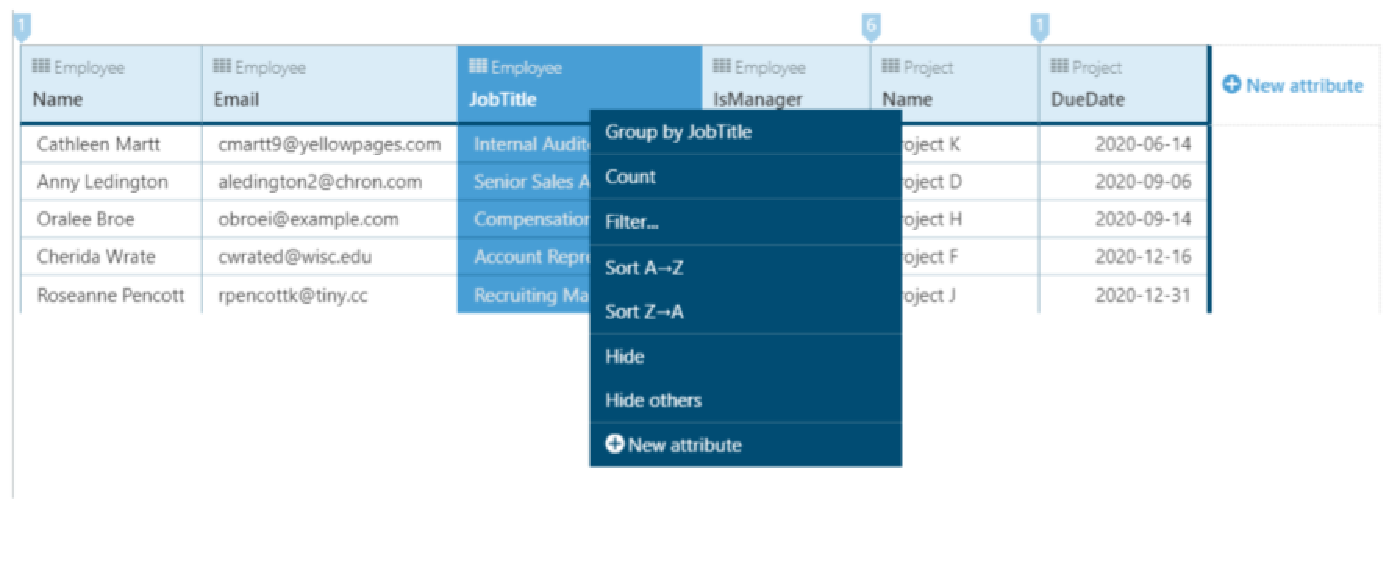
\includegraphics[height=2.3in]{tableRightClickExample}
	\caption{Query Design functions while interacting with Query Result}
	\label{fig:table_right_click_example}
\end{figure}

\begin{figure}[tb]
	\centering
	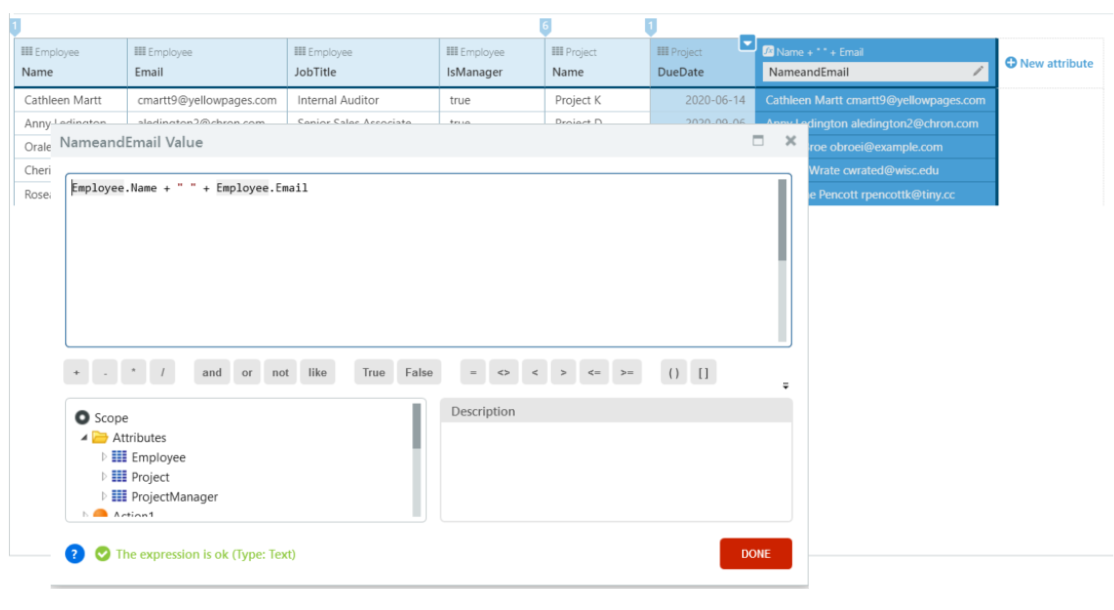
\includegraphics[height=3in]{calculatedAttributeExample}
	\caption{Calculated Attribute Insertion}
	\label{fig:calculated_attribute_example}
\end{figure}


% \begin{figure}[htbp]
% 	\centering
% 	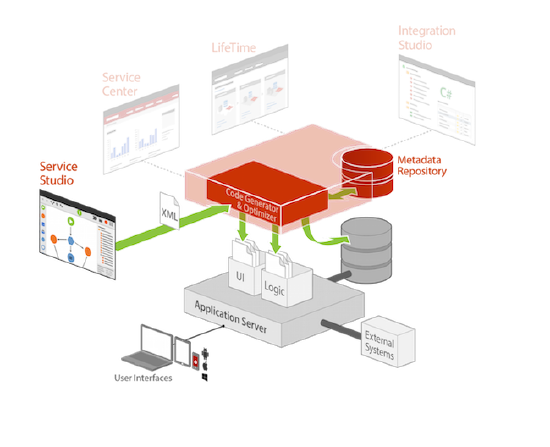
\includegraphics[height=3.75in]{outsystemsArchitecture}
% 	\caption{OutSystems Platform Overview \cite{outsystemsToolsAndComponents}}
% 	\label{fig:outsystemsArchitecture}
% \end{figure}
